\section{Modelo de datos}
	\subsection{Modelo de base de datos}
		\begin{figure}[htbp!]
			\centering
				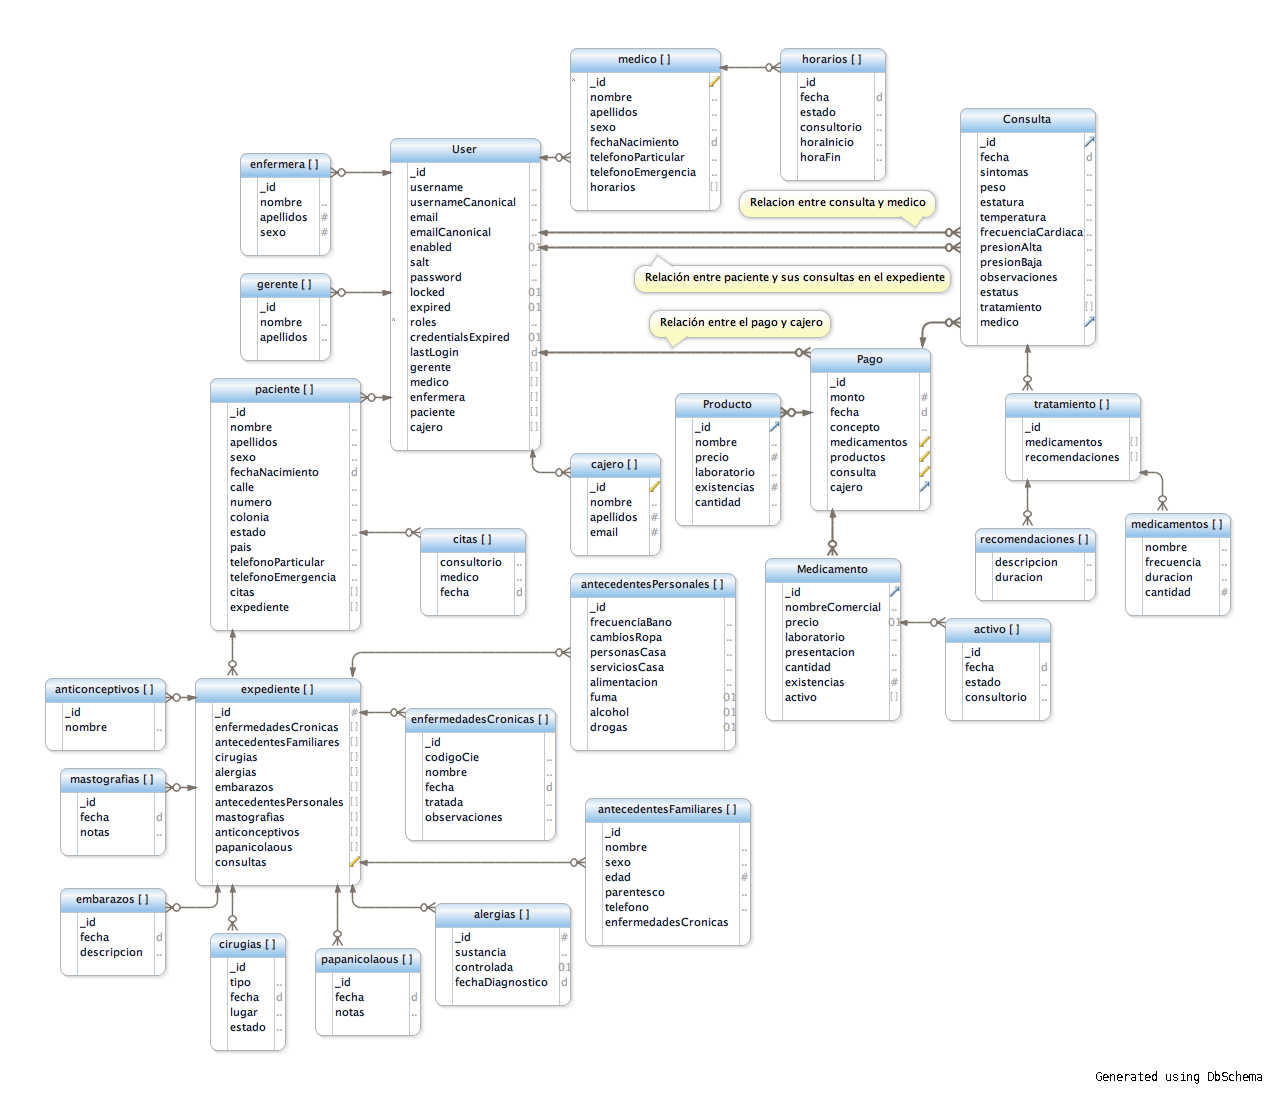
\includegraphics[width=1\textwidth]{images/modeloDatos}
			\caption{Modelo de base de datos}
		\end{figure}
		\newpage
	\subsection{Modelo entidad-relación}
	\newpage
	\subsection{Diccionario de datos}
	\begin{table}[htb]
	\centering
	\begin{tabular}{| p{3.5cm}| p{3.0cm} | p{9.8cm} |}
	\hline
	\multicolumn{3}{|c|}{Colección : User} \\
	\hline
	Campo & Tipo &  Descripción\\ \hline
	\_id & ObjectId & Identificador único de mongodb para el usuario \\ \hline
	username & String & Nombre completo del usuario.\\ \hline
	usernameCanonical & String & Copia del nombre completo del usuario.\\ \hline
	email & String & Email del usuario.\\ \hline
	emailCanonical & String & Copia del email original del usuario.\\ \hline
	enabled & Boolean & Atributo booleano para determinar si el usuario esta habilitado o no.\\ \hline
	salt & String & Número de dígitos aleatorios que se le agregan al hash del password para hacer más segura la contraseña \\ \hline
	password & String & Hash de la contraseña del usuario.\\ \hline
	locked & Boolean & Atributo booleano para determinar si el usuario esta bloqueado o no.\\ \hline
	expired & Boolean & Atributo booleano para determinar si la cuenta del usuario ha expirado. \\ \hline
	roles & Array & Arreglo de roles que tiene el usuario. \\ \hline
	credentialsExpired & Boolean & Atributo booleano para determinar si las credenciales del usuario han expirado. \\ \hline
	lastLogin & Date & Fecha del último login del usuario en el sistema. \\ \hline
	gerente & EmbeddedDocument & Documento embebido para almacenar la información del usuario de tipo gerente \\ \hline
	medico & EmbeddedDocument & Documento embebido para almacenar la información del usuario de tipo \\ \hline
	enfermera & EmbeddedDocument & Documento embebido para almacenar la información del usuario de tipo enfermera \\ \hline
	paciente & EmbeddedDocument & Documento embebido para almacenar la información del usuario de tipo paciente \\ \hline
	cajero & EmbeddedDocument & Documento embebido para almacenar la información del usuario de tipo cajero \\ \hline
	\end{tabular}
	\caption{Tabla de la colección del User.}
	\label{tabla:diccionarioDatos}
	\end{table}
	%=========================================================
	\begin{table}[htb]
	\centering
	\begin{tabular}{| p{3.5cm}| p{3.0cm} | p{9.8cm} |}
	\hline
	\multicolumn{3}{|c|}{Documento embebido : enfermera} \\
	\hline
	Campo & Tipo &  Descripción\\ \hline
	\_id & ObjectId & Identificador único de mongodb para la enfermera \\ \hline
	nombre & String & Nombre(s) de la enfemera.\\ \hline
	apellidos & String & Apellidos de la enfermera.\\ \hline
	sexo & String & Condición orgánica que para distinguir de hombres y mujeres .\\ \hline
	\end{tabular}
	\caption{Tabla del documento embebido de la enfermera .}
	\label{tabla:diccionarioDatos}
	\end{table}
	%=========================================================
	\begin{table}[htb]
	\centering
	\begin{tabular}{| p{3.5cm}| p{3.0cm} | p{9.8cm} |}
	\hline
	\multicolumn{3}{|c|}{Documento embebido : gerente} \\
	\hline
	Campo & Tipo &  Descripción\\ \hline
	\_id & ObjectId & Identificador único de mongodb para el gerente \\ \hline
	nombre & String & Nombre(s) del gerente.\\ \hline
	apellidos & String & Apellidos del gerente.\\ \hline
	\end{tabular}
	\caption{Tabla del documento embebido del gerente .}
	\label{tabla:diccionarioDatos}
	\end{table}
	%=========================================================
	\begin{table}[htb]
	\centering
	\begin{tabular}{| p{3.5cm}| p{3.0cm} | p{9.8cm} |}
	\hline
	\multicolumn{3}{|c|}{Documento embebido : cajero} \\
	\hline
	Campo & Tipo &  Descripción\\ \hline
	\_id & ObjectId & Identificador único de mongodb para el cajero \\ \hline
	nombre & String & Nombre(s) del cajero.\\ \hline
	apellidos & String & Apellidos del cajero.\\ \hline
	\end{tabular}
	\caption{Tabla del documento embebido del cajero .}
	\label{tabla:diccionarioDatos}
	\end{table}
	%=========================================================
	\begin{table}[htb]
	\centering
	\begin{tabular}{| p{3.5cm}| p{3.0cm} | p{9.8cm} |}
	\hline
	\multicolumn{3}{|c|}{Documento embebido : medico} \\
	\hline
	Campo & Tipo &  Descripción\\ \hline
	\_id & ObjectId & Identificador único de mongodb para el médico \\ \hline
	nombre & String & Nombre(s) del médico.\\ \hline
	apellidos & String & Apellidos del médico.\\ \hline
	sexo & String & Condición orgánica que para distinguir de hombres y mujeres .\\ \hline
	fechaNacimiento & Date &  Fecha de nacimiento del médico.\\ \hline
	telefonoParticular & String & Telefono particular para contactar al médico.\\ \hline
	telefonoEmergencia & String & Telefono de emergencia para contactar al médico.\\ \hline
	horarios & EmbeddedDocument(s) &  Documento(s) embebido(s) para almacenar la información pertinente al horario de servicio del médico.\\ \hline

	\end{tabular}
	\caption{Tabla del documento embebido del médico .}
	\label{tabla:diccionarioDatos}
	\end{table}
	%=========================================================
	\begin{table}[htb]
	\centering
	\begin{tabular}{| p{3.5cm}| p{3.0cm} | p{9.8cm} |}
	\hline
	\multicolumn{3}{|c|}{Documento embebido : paciente} \\
	\hline
	Campo & Tipo &  Descripción\\ \hline
	\_id & ObjectId & Identificador único de mongodb para el paciente \\ \hline
	nombre & String & Nombre(s) del médico.\\ \hline
	apellidos & String & Apellidos del médico.\\ \hline
	sexo & String & Condición orgánica que para distinguir de hombres y mujeres .\\ \hline
	fechaNacimiento & Date &  Fecha de nacimiento del paciente.\\ \hline
	calle & String & Calle del \textit{domicilio donde reside }el paciente actualmente\\ \hline
	numero & String & Telefono de emergencia para contactar al médico.\\ \hline
	citas & EmbeddedDocument(s) &  Documento(s) embebido(s) para almacenar la información pertinente a las citas del paciente.\\ \hline

	\end{tabular}
	\caption{Tabla del documento embebido del paciente .}
	\label{tabla:diccionarioDatos}
	\end{table}
	
	
	\begin{table}[htb]
	\centering
	\begin{tabular}{| p{3.5cm}| p{3.0cm} | p{9.8cm} |}
	\hline
	\multicolumn{3}{|c|}{Colección : Consulta} \\
	\hline
	Campo & Tipo &  Descripción\\ \hline
	
	\_id & ObjectId & Identificador único de mongodb para la Consulta \\ \hline
	fecha  & Date & Fecha en la que está siendo atendida la consulta 	\\ \hline
	sintomas & String & Sintomas que presenta el paciente.\\ \hline
	peso & String & Peso medido en kg del paciente \\ \hline
		estatura & String & Estatura medida en metros y centimetros del paciente\\ \hline
		temperatura & String & Temperatura que presenta el paciente medida en grados centigrados. \\ \hline
		frecuenciaCardiaca & String & Frecuencia cardiaca que presenta el paciente \\ \hline
		PresionAlta & String &  número flotante: medido en ``mm de Hg”  (míımetros de mercurio), límite superior de la presión del paciente. \\ \hline
		presionBaja & String &  número flotante: medido en ``mm de Hg”  (míımetros de mercurio), límite inferior de la presión del paciente. \\ \hline
		observaciones & String & Observaciones que describen la situación de salud del paciente \\ \hline
		estatus & String & Describe el estado de la consulta, pagada, en espera, siendo atendida.  \\ \hline
		tratamiento & EmbebedDocument & Documento embebido para almacenar la información del tratamiento. \\ \hline
		medico & ReferenceOne & almacena el id del médico que impartió la cita \\ \hline
	
	\end{tabular}
	\caption{Tabla de la colección de consulta .}
	\label{tabla:diccionarioDatos}
	\end{table}



\begin{table}[htb]
	\centering
	\begin{tabular}{| p{3.5cm}| p{3.0cm} | p{9.8cm} |}
	\hline
	\multicolumn{3}{|c|}{Documento embebido :Tratamiento} \\
	\hline
	Campo & Tipo &  Descripción\\ \hline
	
	\_id & ObjectId & Identificador único de mongodb para el tratamiento \\ \hline
	medicamento & EmbebedDocuments & Documento(s) embebido(s) para almacenar los medicamentos recetados en el tratamiento. \\ \hline
	
	recomedaciones & EmbebedDocuments & Documento(s) embebido(s) para almacenar las recomendaciones del  en el tratamiento. \\ \hline
	
	\end{tabular}
	\caption{Tabla del documento embebido Tratamiento .}
	\label{tabla:diccionarioDatos}
	\end{table}


\begin{table}[htb]
	\centering
	\begin{tabular}{| p{3.5cm}| p{3.0cm} | p{9.8cm} |}
	\hline
	\multicolumn{3}{|c|}{Documento embebido :Medicamentos} \\
	\hline
	Campo & Tipo &  Descripción\\ \hline
		
	nombre & String & Nombre del medicamento que será recetado \\ \hline
	frecuencia & String & Frecuencia de uso del medicamento recetado \\ \hline
	duracion & String & Tiempo que el paciente debe tomar el medicamento\\ \hline
	cantidad & String & Cantidad del medicamento que el paciente debe comprar	\\ \hline
	
	\end{tabular}
	\caption{Tabla del documento embebido Medicamento .}
	\label{tabla:diccionarioDatos}
	\end{table}


\begin{table}[htb]
	\centering
	\begin{tabular}{| p{3.5cm}| p{3.0cm} | p{9.8cm} |}
	\hline
	\multicolumn{3}{|c|}{Documento embebido :Recomendacion} \\
	\hline
	Campo & Tipo &  Descripción\\ \hline
	
	
	
	descripción & String & Descripción extensa de lo que el paciente debe hacer para mejorar su estado de salud \\ \hline
	duracion & String & Tiempo que el paciente debe seguir la recomendación \\ \hline
	
	
	\end{tabular}
	\caption{Tabla del documento embebido Recomendación .}
	\label{tabla:diccionarioDatos}
	\end{table}
	
	
	
\begin{table}[htb]
	\centering
	\begin{tabular}{| p{3.5cm}| p{3.0cm} | p{9.8cm} |}
	\hline
	\multicolumn{3}{|c|}{Documento embebido :Alergia} \\
	\hline
	Campo & Tipo &  Descripción\\ \hline
	
	\_ id & Objectid &identificador únido de mongodb para la alergia \\ \hline
	sustancia & String & Sustancia a la que es alergico el paciente \\ \hline
	controlada & Boolean & Describe si es tratada o no \\ \hline 
	fechaDiagnosticada & Date & Describe la fecha en la que fue diagnosticada la alergia \\ \hline

	
	\end{tabular}
	\caption{Tabla del documento embebido Alergia .}
	\label{tabla:diccionarioDatos}
	\end{table}

\begin{table}[htb]
	\centering
	\begin{tabular}{| p{3.5cm}| p{3.0cm} | p{9.8cm} |}
	\hline
	\multicolumn{3}{|c|}{Documento embebido :AntecedenteFamiliar} \\
	\hline
	Campo & Tipo &  Descripción\\ \hline
	
	\_ id & Objectid &identificador únido de mongodb para el antecedente \\ \hline
	
	nombre & String & Nombre de la persona con parentesco familiar  \\ \hline
	
	sexo &  String & Describe el sexo de la persona con parentesco familiar \\ \hline
	
	edad & int & Describe la edad de la persona con parentesco familiar \\ \hline
	
	parentesco & String & Describe que relación familiar tiene con el paciente \\ \hline
	
	telefono & String & Almacena el telefono de la persona con parentesco familiar \\ \hline
	
	controlada & Boolean & almacena si la enfermedad es tratada o no \\ \hline
	
	fechaDiagnostico & Date  & almacena la fecha en la que fue diagnosticada la enfermedad para el familiar \\ \hline
	
	enfermedadesCronicas & EmbebedDocument & Documento(s) embebido(s) para almacenar una lista de enfermedades cronicas \\ \hline
	
	\end{tabular}
	\caption{Tabla del documento embebido AntecedenteFamiliar .}
	\label{tabla:diccionarioDatos}
	\end{table}


\begin{table}[htb]
	\centering
	\begin{tabular}{| p{3.5cm}| p{3.0cm} | p{9.8cm} |}
	\hline
	\multicolumn{3}{|c|}{Documento embebido :AntecedentePersonal} \\
	\hline
	Campo & Tipo &  Descripción\\ \hline
	
	\_ id & Objectid &identificador únido de mongodb para el antecedente \\ \hline
	
	frecuenciaBano & String & Almacena cuantas veces se baña  \\ \hline
	
	cambiosRopa &  String & Almacena el número de veces que hace cambio de ropa\\ \hline
	
	personasCasa & String & Almacena el número de personas que viven en la misma casa con el paciente \\ \hline
	
	serviciosCasa & array & Arreglo de servicios que tiene la casa. \\ \hline
	
	alimentación & String & Describe que tipo de alimentación lleva el paciente (Buena, regular, mala)\\ \hline
	
	fuma & Boolean & almacena si el paciente fuma o no\\ \hline
	
	alcohol & Boolean  & almacena si el paciente toma alcohol o no \\ \hline
	
	drogas & Boolean & Almacena si el paciente consume drogas o no \\ \hline
	
	\end{tabular}
	\caption{Tabla del documento embebido AntecedentePersonal .}
	\label{tabla:diccionarioDatos}
	\end{table}
	
	
	\begin{table}[htb]
	\centering
	\begin{tabular}{| p{3.5cm}| p{3.0cm} | p{9.8cm} |}
	\hline
	\multicolumn{3}{|c|}{Documento embebido :Anticonceptivo} \\
	\hline
	Campo & Tipo &  Descripción\\ \hline
	
	\_ id & Objectid &identificador únido de mongodb para el anticonceptivo \\ \hline
	
	nombre & String & Almacena el nombre del anticonceptivo.

	\end{tabular}
	\caption{Tabla del documento embebido Anticonceptivo .}
	\label{tabla:diccionarioDatos}
	\end{table}



	\begin{table}[htb]
	\centering
	\begin{tabular}{| p{3.5cm}| p{3.0cm} | p{9.8cm} |}
	\hline
	\multicolumn{3}{|c|}{Documento embebido :Cirugia} \\
	\hline
	Campo & Tipo &  Descripción\\ \hline
	
	\_ id & Objectid &identificador únido de mongodb para la cirugia \\ \hline
	
	tipo & String & Almacena el tipo de cirugia que el paciente recibió \\ \hline
	
	fecha & Date & Almacena la fecha en la que fue realizada dicha cirugia \\ \hline
	
	lugar & String & Almacena el lugar donde fue realizada dicha cirugia (hospital) \\ \hline
	
		
	Estado & String & Almacena el estado donde fue realizada dicha cirugia \\ \hline
	

	\end{tabular}
	\caption{Tabla del documento embebido Cirugia .}
	\label{tabla:diccionarioDatos}
	\end{table}


	\begin{table}[htb]
	\centering
	\begin{tabular}{| p{3.5cm}| p{3.0cm} | p{9.8cm} |}
	\hline
	\multicolumn{3}{|c|}{Documento embebido :Embarazo} \\
	\hline
	Campo & Tipo &  Descripción\\ \hline
	
	\_ id & Objectid &identificador únido de mongodb para el embarazo \\ \hline
	
	fecha & Date & Almacena la fecha del embarazo.
	\\ \hline
	descripcion & String & Proporciona una breve descripción del embarazo. 

	\end{tabular}
	\caption{Tabla del documento embebido Embarazo .}
	\label{tabla:diccionarioDatos}
	\end{table}
	
	
	\begin{table}[htb]
	\centering
	\begin{tabular}{| p{3.5cm}| p{3.0cm} | p{9.8cm} |}
	\hline
	\multicolumn{3}{|c|}{Documento embebido :Enfermedad} \\
	\hline
	Campo & Tipo &  Descripción\\ \hline
	
	\_ id & Objectid &identificador únido de mongodb para la enfermedad \\ \hline
	
	codigoCie & String & Código único para clasificación de la enfermedad \\ \hline
	
	nombre & String & Nombre de la enfermedad \\ \hline	
	
	fecha & Date & Almacena la fecha en la que fue diagnosticada la enfermedad.
	\\ \hline
	
	tratada & Boolean & Almacena si la enfermedad está siendo o no tratada. \\ \hline	
	
	observaciones & String & Proporciona una breve descripción hecha por el médico acerca de la enfermedad. \\ \hline 

	\end{tabular}
	\caption{Tabla del documento embebido Embarazo .}
	\label{tabla:diccionarioDatos}
	\end{table}
	
	
	
	
	\begin{table}[htb]
	\centering
	\begin{tabular}{| p{3.5cm}| p{3.0cm} | p{9.8cm} |}
	\hline
	\multicolumn{3}{|c|}{Documento embebido :Mastografia} \\
	\hline
	Campo & Tipo &  Descripción\\ \hline
	
	\_ id & Objectid &identificador únido de mongodb para la mastografía  \\ \hline
	
	fecha & Date & Almacena la fecha en la que fue realizada la mastografía.
	\\ \hline
	notas & String & Proporciona una breve descripción de la mastografía.  \\ \hline

	\end{tabular}
	\caption{Tabla del documento embebido Mastografía .}
	\label{tabla:diccionarioDatos}
	\end{table}
	
	
	
	
	
	
	
	
	 \clearpage
	 
	 \begin{table}[htb]
	\centering
	\begin{tabular}{| p{3.5cm}| p{3.0cm} | p{9.8cm} |}
	\hline
	\multicolumn{3}{|c|}{Documento embebido :Papanicolaou} \\
	\hline
	Campo & Tipo &  Descripción\\ \hline
	
	\_ id & Objectid &identificador únido de mongodb para el papanicolaou  \\ \hline
	
	fecha & Date & Almacena la fecha en la que fue realizado el papanicolaou.
	\\ \hline
	notas & String & Proporciona una breve descripción del papanicolaou.  \\ \hline

	\end{tabular}
	\caption{Tabla del documento embebido Papanicolaou .}
	\label{tabla:diccionarioDatos}
	\end{table}
	 
	 
	 \begin{table}[htb]
	\centering
	\begin{tabular}{| p{3.5cm}| p{3.0cm} | p{9.8cm} |}
	\hline
	\multicolumn{3}{|c|}{Documento embebido :Expediente} \\
	\hline
	Campo & Tipo &  Descripción\\ \hline
	
	\_ id & Objectid &identificador únido de mongodb para el expediente  \\ \hline
	
	enfermedadesCronicas & EmbebedDocument & Documento(s) embebidos que almancenan una lista de enfermedades cronicas \\ \hline
	
	antecedentesFamiliares& EmbebedDocument & Documento(s) embebidos que almancenan una lista de antecedentes familiares\\ \hline
	
	cirugias & EmbebedDocument & Documento(s) embebidos que almancenan una lista de cirugías\\ \hline
	
	alergias & EmbebedDocument & Documento(s) embebidos que almancenan una lista de alergías \\ \hline
	
	embarazos & EmbebedDocument & Documento(s) embebidos que almancenan una lista de embarazos \\ \hline
	
	antecedentesPersonales & EmbebedDocument & Documento(s) embebidos que almancenan una lista de antecedentes personales \\ \hline
	
	anticoncepctivos & EmbebedDocument & Documento(s) embebidos que almancenan una lista de anticonceptivos usados con frecuencia\\ \hline
	
	mastografias & EmbebedDocument & Documento(s) embebidos que almancenan una lista de mastografías tenidas \\ \hline
	
	papanicolaous & EmbebedDocument & Documento(s) embebidos que almancenan una lista de papanicolaous tenidos\\ \hline
	
	consultas & EmbebedDocument & Documento(s) embebidos que almancenan una lista de consultas tenidas\\ \hline
			
	
	\end{tabular}
	\caption{Tabla del documento embebido Expediente .}
	\label{tabla:diccionarioDatos}
	\end{table}	 
	 
	 
	 
	 \begin{table}[htb]
		\centering
		\begin{tabular}{| p{3.5cm}| p{3.0cm} | p{9.8cm} |}
			\hline
			\multicolumn{3}{|c|}{Colección : Pago} \\
			\hline
			Campo & Tipo &  Descripción\\ \hline
			\_id & ObjectId & Identificador único de mongodb para el pago. \\ \hline
			monto & float & Costo total del pago.\\ \hline
			fecha & timestamp & Fecha y hora de registro del pago.\\ \hline
			concepto & String & Pequeña descripción del pago.\\ \hline
			medicamentos & EmbeddedDocument & Documento embebido para almacenar la información de los medicamentos del pago (Consulte Colección : Medicamento). \\ \hline
			productos & EmbeddedDocument & Documento embebido para almacenar la información de los productos del pago (Consulte Colección : Producto). \\ \hline
			consulta & EmbeddedDocument & Documento embebido para almacenar la información de las consultas del pago (Consulte Colección : Consulta). \\ \hline
			cajero & EmbeddedDocument & Documento embebido para almacenar la información del cajero que registró el pago (Consulte Documento embebido : Cajero). \\ \hline
		\end{tabular}
		\caption{Tabla de la colección de Pago.}
		\label{tabla:diccionarioDatos}
	\end{table}
	
	\begin{table}[htb]
		\centering
		\begin{tabular}{| p{3.5cm}| p{3.0cm} | p{9.8cm} |}
			\hline
			\multicolumn{3}{|c|}{Colección : Producto} \\
			\hline
			Campo & Tipo &  Descripción\\ \hline
			\_id & ObjectId & Identificador único de mongodb para el producto. \\ \hline
			nombre & String & Nombre del producto.\\ \hline
			precio & float & Precio unitario del producto.\\ \hline
			laboratorio & String & Laboratorio que fabrica el producto.\\ \hline
			existencias & int & Cantidad de productos disponibles en inventario.\\ \hline
			cantidad & float & Tamaño del contenido del producto.\\ \hline
		\end{tabular}
		\caption{Tabla de la colección de Producto.}
		\label{tabla:diccionarioDatos}
	\end{table}
	
	
	\begin{table}[htb]
		\centering
		\begin{tabular}{| p{3.5cm}| p{3.0cm} | p{9.8cm} |}
			\hline
			\multicolumn{3}{|c|}{Colección : Medicamento} \\
			\hline
			Campo & Tipo &  Descripción\\ \hline
			\_id & ObjectId & Identificador único de mongodb para el medicamento. \\ \hline
			nombreComercial & String & Nombre comercial del medicamento.\\ \hline
			precio & float & Precio unitario del medicamento.\\ \hline
			laboratorio & String & Laboratorio que fabrica el medicamento.\\ \hline
			presentacion & String & Unidades del medicamento (ml, mg, tabletas, etc.).\\ \hline
			cantidad & float & Tamaño del contenido del producto.\\ \hline
			exitencias & int & Cantidad de medicamentos disponibles en inventario.\\ \hline			
			activos & EmbeddedDocument & Documento embebido para almacenar la información de los ingredientes activos del medicamento (Consulte Documento embebido: Activo). \\ \hline
		\end{tabular}
		\caption{Tabla de la colección de Medicamento.}
		\label{tabla:diccionarioDatos}
	\end{table}
	
	
	\begin{table}[htb]
		\centering
		\begin{tabular}{| p{3.5cm}| p{3.0cm} | p{9.8cm} |}
			\hline
			\multicolumn{3}{|c|}{Documento embebido : Activo} \\
			\hline
			Campo & Tipo &  Descripción\\ \hline
			\_id & ObjectId & Identificador único de mongodb para el ingrediente activo. \\ \hline
			nombre & String & Nombre del ingrediente activo.\\ \hline
			cantidad & float & Cantidad del ingrediente activo en el medicamento.\\ \hline
			
		\end{tabular}
		\caption{Tabla del documento embebido del ingrediente activo .}
		\label{tabla:diccionarioDatos}
	\end{table}
	
		\newpage

	






	%=========================================================


\section{Modelo de acceso de datos}


